\documentclass[12pt]{article}
\usepackage[utf8]{inputenc}
\usepackage[french]{babel}
\usepackage[a4paper,left=2cm,right=2cm,top=2cm,bottom=2cm]{geometry}
\usepackage{indentfirst}
\usepackage{appendix}
\usepackage{libertine}
\usepackage{titlesec}
\usepackage{eso-pic}
\usepackage{fancyhdr}
\usepackage{graphicx}
\usepackage{wrapfig}
\usepackage{float}
\usepackage{caption}
\usepackage{color}
\usepackage{setspace}
\usepackage[T1]{fontenc}
\usepackage[hyphens]{url}
\usepackage[backend=bibtex,style=alphabetic]{biblatex}
\addbibresource{source.bib}\usepackage[linkbordercolor=white]{hyperref}
\usepackage{hyperref}
\usepackage{caption}
\usepackage{subcaption}
\usepackage{bm}
\usepackage{enumitem}
\usepackage{siunitx}
\usepackage{textcomp}
\usepackage{amsmath}
\usepackage{commath}
\usepackage{cancel}
\usepackage{pdflscape}
\usepackage{svg}
\usepackage[linesnumbered,ruled,vlined]{algorithm2e} % Retain only one package
\usepackage{comment}
\usepackage{placeins}
\usepackage{listings}
\lstset{literate=%
    {à}{{\`a}}1 {â}{{\^a}}1 {é}{{\'e}}1 {è}{{\`e}}1 {ê}{{\^e}}1 {ë}{{\"e}}1 {î}{{\^i}}1 {ï}{{\"i}}1 {ô}{{\^o}}1 {ö}{{\"o}}1 {ù}{{\`u}}1 {û}{{\^u}}1 {ü}{{\"u}}1 {ç}{{\c{c}}}1 {Ç}{{\c{C}}}1{―}{{\textemdash}}1
    {’}{{'}}1 {‘}{{`}}1 {“}{{``}}1 {”}{{''}}1
}
\urlstyle{same}
\pagestyle{fancy}
\fancyhead[L]{\leftmark}
\fancyhead[R]{}
\renewcommand{\subsectionmark}[1]{}


\usepackage{titlesec}
\usepackage{hyperref}

\titleclass{\subsubsubsection}{straight}[\subsection]


\newcounter{subsubsubsection}[subsubsection]
\renewcommand\thesubsubsubsection{\thesubsubsection.\arabic{subsubsubsection}}
\renewcommand\theparagraph{\thesubsubsubsection.\arabic{paragraph}} % optional; useful if paragraphs are to be numbered


\titleformat{\subsubsubsection}
  {\normalfont\normalsize\bfseries}{\thesubsubsubsection}{1em}{}
\titlespacing*{\subsubsubsection}
{0pt}{3.25ex plus 1ex minus .2ex}{1.5ex plus .2ex}
\makeatletter
\renewcommand\paragraph{\@startsection{paragraph}{5}{\z@}%
  {3.25ex \@plus1ex \@minus.2ex}%
  {-1em}%
  {\normalfont\normalsize\bfseries}}
\renewcommand\subparagraph{\@startsection{subparagraph}{6}{\parindent}%
  {3.25ex \@plus1ex \@minus .2ex}%
  {-1em}%
  {\normalfont\normalsize\bfseries}}
\def\toclevel@subsubsubsection{4}
\def\toclevel@paragraph{5}
\def\toclevel@paragraph{6}
\def\l@subsubsubsection{\@dottedtocline{4}{7em}{4em}}
\def\l@paragraph{\@dottedtocline{5}{10em}{5em}}
\def\l@subparagraph{\@dottedtocline{6}{14em}{6em}}
\makeatother
\setcounter{secnumdepth}{4}
\setcounter{tocdepth}{4}

\setlength{\headheight}{14.5pt}
\setlength{\parskip}{1em}
\renewcommand{\baselinestretch}{0.6}
\renewcommand{\headrulewidth}{1pt}
\newcommand{\HRule}{\rule{\linewidth}{0.3mm}}
\newcommand\BackgroundPic{%
	\put(0,0){%
		\parbox[b][\paperheight]{\paperwidth}{%
			\vfill
			\centering
			
\includegraphics[width=\paperwidth,height=\paperheight,%
			keepaspectratio]{background.png}%
			\vfill}}}

% -----------------------------------------------------


\begin{document}
\AddToShipoutPicture*{\BackgroundPic}
\begin{titlepage}
  \begin{sffamily}
  \begin{flushleft} \large
    
\includegraphics[height=2.0cm]{logo_ulb.jpg}
    \vspace{5cm}
   \end{flushleft}
  \begin{center}

    %Title
	\textsc{\huge INFO-F203 - Projets d'algorithmique 2}\\[1cm]

    \HRule \\[0.7cm]

	\textsc {\Huge Projet Mobilité}\\[0.4cm]

    \HRule \\[1.2cm]

% Author and supervisor
\begin{minipage}{0.5\textwidth}
\begin{flushleft} \large
\emph{Auteurs:}\\
Romain \textsc{Liefferinckx} - 000591790\\
Manuel \textsc{Rocca} - 000596086\\


\end{flushleft}
\end{minipage}


\begin{minipage}{0.4\textwidth}
\begin{flushright} \large
\emph{Professeurs:} \\
Jean  \textsc{Cardinal}\\
\emph{Assistants:} \\
Robin \textsc{Petit}
\end{flushright}
\end{minipage}


    \vfill

    %Bottom of the page
    {\large Année académique 2024-2025}
  \end{center}

  \end{sffamily}
\end{titlepage}


\clearpage


\tableofcontents

\newpage

% -----------------------------------------------------

\section{Introduction}
Dans le cadre de notre cours d'algorithmique INFO F-203, l'occasion s'est présentée à nous de créer un programme cherchant un chemin optimal
entre un point A et un point B sur base d'une heure de départ. En effet, sur base d'un ensemble de données
fournies sous format \emph{General Transit Feed Specification} (\textbf{GTFS}), nous avons utilisé le \emph{Connexion Scan Algorithm} (\textbf{CSA})
pour implémenter notre chercheur de chemin en \emph{Java}. 

Dans les sections à suivre, nous abordons l'initialisation des données, des structures formées à partir de celles-ci pour notre
implémentation et certains détails techniques comme la complexité temporelle et spatiale. Nous justifierons également certains choix
comme celui de l'algorithme précisé ci-dessus, à savoir le \textbf{CSA}.


\section{Initialisation des données}
\label{sec:init}
Dans cette section nous expliquons les procédés utilisés pour charger les données en mémoire à partir des fichiers CSV fournis ainsi que
les structures de données utilisées pour leur stockage et leur utilisation optimale dans l'algorithme choisi par nos soins.

Tout d'abord, décrivons brièvement la classe Parser, qui se charge de la lecture des fichiers CSV et de la création de dictionnaires (\emph{HashMap}) contenant les données chargées, faciles d'accès.
Nous avons créé, pour chaque type de fichier CSV, une classe de stockage qui contient les attributs correspondants aux champs du fichier CSV. Quelques subtilités notables au sujet de ces classes sont
décrites dans les sections suivantes.

\subsection{Objets de base pour le stockage}
Les fichiers CSV fournis contiennent des informations sur les arrêts, les trajets, les horaires et les routes de quatre entreprises de transport en commun,
à savoir la STIB en région Bruxelloise, TEC en région Wallone, DELIJN en région FLamande et, finalement, la SNCB pour le transport ferroviaire au niveau national.

Pour chaque type de fichier CSV, voici donc les classes correspondantes créées pour contenir les données de manière accessible.

\subsubsection{La classe Route}
Cette classe est une simple classe de stockage, chaque attribut correspondant à un champ des fichiers \emph{routes.csv}.

% Table qui détaille la classe Route
\begin{table}[h]
    \centering
    \begin{tabular}{|l|l|p{8cm}|}
    \hline
    \textbf{Attribut} & \textbf{Type} & \textbf{Description} \\
    \hline
    routeId & final String & L'identifiant de la route représentée \\
    routeShortName & final String & Le nom de la route raccourci \\
    routeLongName & final String & Le nom de la route complet \\
    routeType & final String & Le type de véhicule utilisant cette route \\
    \hline
    \end{tabular}
    \caption{Classe Route}
\end{table}

\subsubsection{La classe StopTime}
La particularité de cette classe est qu'il lui manque le champ trip\_id donné dans les CSV concernés. Ce choix découle
de la structure de la classe Trip détaillée dans la section \hyperref[sec:trip]{2.1.4}.
% Table qui détaille la classe StopTime
\begin{table}[h]
    \centering
    \begin{tabular}{|l|l|p{8cm}|}
    \hline
    \textbf{Attribut} & \textbf{Type} & \textbf{Description} \\
    \hline
    departureTime & final int & L'heure du départ à partir de
                                   l'arrêt associé sur le trajet associé en format 
                                   heure;minutes;secondes \\
    stopId & final String & L'identifiant de l'arrêt associé \\
    stopSequence & final int & Le numéro de l'arrêt dans le trajet associé \\
    \hline
    \end{tabular}
    \caption{Classe StopTime}
\end{table}

\subsubsection{La classe Stop}
Dans cette classe, hormis le fait que chaque champ des fichiers \emph{routes.csv} est repris, nous avons fait le choix d'ajouter
une liste d'identifiants de trajet, permettant de retrouver efficacement chaque trajet partant de cet arrêt ainsi qu'une liste de \hyperref[sec:walk]{\emph{Walk}}, permettantd'avoir un accès rapide à tous les arrêts accessibles à pied depuis cet arrêt.

Cette classe comprend également une méthode \emph{getDistanceToOther} qui permet de calculer la distance entre deux arrêts en utilisant la formule de Haversine,
implémentée dans une classe annexe, la classe \emph{Calculator}.

% Table qui détaille la classe Stop
\begin{table}[h]
    \centering
    \begin{tabular}{|l|l|p{8cm}|}
    \hline
    \textbf{Attribut} & \textbf{Type} & \textbf{Description} \\
    \hline
    stopId & final String & L'identifiant du stop représenté \\
    stopName & final String & Le nom du stop \\
    stopLat & final String & La latitude du stop \\
    stopLon & final String & La longitude du stop \\
    tripIds & List$<$String$>$ & La liste des tous les trips (leurs identifiants) partant de ce stop \\
    walks & List$<$Walk$>$ & La liste de tous les arrêts accessibles à pied depuis ce stop \\
    \hline
    \end{tabular}
    \caption{Classe Stop}
\end{table}

\subsubsection{La classe Trip}
\label{sec:trip}
Une fois de plus, en plus des champs trouvés dans les fichiers \emph{trips.csv} retranscrits en attribut, nous avons ajouté
une liste d'heures d'arrêt associés à ce trajet. Ceci nous permet de construire efficacement les connexions entre arrêts affublées
de temps de départ et d'arrivée.

% Table qui détaille la classe Trip
\begin{table}[h]
    \centering
    \begin{tabular}{|l|l|p{8cm}|}
    \hline
    \textbf{Attribut} & \textbf{Type} & \textbf{Description} \\
    \hline
    tripId & final String & L'identifiant du trip représenté \\
    routeId & final String & L'identifiant de la route sur laquelle il passe \\
    stopTimes & List$<$StopTime$>$ &  La liste de tous les StopTime associés à ce trip \\
    \hline
    \end{tabular}
    \caption{Classe Trip}
\end{table}

\subsection{Création des structures de données}
Une fois les données lues et contenues dans des dictionnaires faciles d'accès (accès en temps constant), nous procédons à la création de structures de données
pertinentes à notre algorithme de recherche de chemin, le CSA à l'aide de la classe Builder.

La classe Builder est responsable de la création d'une liste de connexions entre arrêts, de la création du BallTree utilisé pour construire efficacement les transferts à pied entre arrêts
et, finalement, la création de ces transferts à pied.

\subsubsection{La classe Connexion}
L'algorithme CSA se base, comme son nom l'indique, sur des connexions entre les différents arrêts. Pour traiter cet aspect, nous avons fait le choix logique
d'implémenter une classe \emph{Connexion}.

\begin{table}[h]
    \centering
    \begin{tabular}{|l|l|p{8cm}|}
    \hline
    \textbf{Attribut} & \textbf{Type} & \textbf{Description} \\
    \hline
    tripId & final String & L'identifiant du trajet utilisé par la connexion \\
    fromId & final String & L'identifiant de l'arrêt de de départ \\
    toId & final String &  L'identifiant de l'arrêt d'arrivée \\
    departureTime & final int & L'heure de départ de l'arrêt \emph{fromId} \\
    arrivalTime & final int & L'heure d'arrivée à l'arrêt \emph{toId} \\
    \hline
    \end{tabular}
    \caption{Classe Trip}
\end{table}


\subsubsection{La classe BallTree}
Afin de construire les transferts à pied (limités à une distance arbitraire), nous avons d'abord commencé par une implémentation brute-force en itérant, pour chaque arrêt, sur tous les
autres arrêts en $O(n^2)$, $n$ étant le nombre d'arrêts. Cependant, avec un total d'environ 65 000 arrêts, cette approche impliquait environ 4,5 milliards d'itérations avec, à chaque 
itération, une série d'opérations comme par exemple le calcul de la distance entre deux arrêts, en temps constant. Ceci nous a mené à un temps d'exécution d'environ 10 minutes sur nos 
machines rien que pour la création de ces transferts à pied, ce qui est, vous en conviendrez, absolument inacceptable.

Afin de remédier à ce problème critique, nous nous sommes penchés sur des structures de données plus adaptées à ce type de problème. Suite à une série de recherches et discussions avec
nos collègues, nous avons opté pour le \emph{BallTree}, une structure de données arborescente où chaque nœud représente une boule dans l'espace N-dimensionnel contenant un sous-ensemble d'arrêts.
Cette structure permet de récupérer efficacement les voisins d'un arrêts donné dans un rayon donné à l'aide de requêtes rapides.

\subsubsection{La classe Walk}
\label{sec:walk}
Classe simple, représentant un transfert à pied entre deux arrêts. Ces objets sont contenus sous forme de liste dans les arrêts correspondants.

\begin{table}[h]
    \centering
    \begin{tabular}{|l|l|p{8cm}|}
    \hline
    \textbf{Attribut} & \textbf{Type} & \textbf{Description} \\
    \hline
    departure & final Stop & L'arrêt de départ du transfert à pied \\
    destination & final Stop & L'arrêt d'arrivée du transfert à pied \\
    duration & final int & La durée en secondes du transfert à pied \\
    \hline
    \end{tabular}
    \caption{Classe Walk}
\end{table}

\newpage
\subsection{Complexité de l'initialisation}
Bien qu'étant une étape antérieure à l'exécution de l'algorithme, il reste important de discuter la complexité de cette étape. En effet, si nous avions choisi d'absolument ignorer
l'aspect de la complexité, nous aurions pu rester sur une implémentation brute-force, prenant 10 minutes à l'exécution. Bien entendu, pour éviter ces absurdités, nous avons apporté
un soin particulier à la création de ces structures de données.

\subsubsection{Complexité temporelle}
\label{sec:complexitetempinit}
L'initialisation des données se fait en plusieurs étapes, chacune ayant sa propre complexité. Premièrement, nous avons la lecture des fichiers CSV, qui a naturellement une complexité
linéaire $O(n)$, où $n$ est le nombre de lignes dans le fichier. 

Ensuite, pour la création des connexions, nous itérons dans tous les trajets et, pour chaque trajet, nous itérons dans leurs heures d'arrêts associés. Notons $n$ le nombre de trajets et $m$ le 
nombre d'arrêts associés à chaque trajet. La complexité de cette étape est donc $O(n \cdot m)$. Une fois la liste de connexions créée, nous procédons au tri de celle-ci en se basant sur 
l'heure de départ de chaque connexion à l'aide de l'algorithme de tri \emph{TimSort}, utilisé par \emph{Collections.sort()}. Ceci se fait dans les pires et
moyen cas avec une complexité de $O(n \log n)$, où $n$ est le nombre de connexions avec un meilleur cas s'exécutant en $O(n)$ (si la liste est déjà majoritairement triée).

Finalement, le plus intéressant, la construction du \emph{BallTree} et des transferts à pied. La construction de notre \emph{BallTree} se fait de manière récursive, en divisant à chaque appel 
récursif l'ensemble des arrêts en deux sous-ensembles. Pour ce faire, des méthodes annexes comme \emph{FindFarthest} ou \emph{ComputeCenter} sont utilisées. Chacune d'entre elles s'exécute en 
temps linéaire, $O(n)$, où $n$ est le nombre d'arrêts dans l'ensemble de données. Quatres fonctions linéaires sont executées à chaque appel récursif, ce qui nous amène à une complexité de 
$4 * O(n)$, ce que nous pouvons résumer à $O(n)$. Finalement, concernant les appels récursifs, en supposant le partitionnement parfait, nous avons une profondeur d'arbre de $\log n$ et donc 
$O(n \log n)$ pour la construction de l'arbre complet.

Suite à quelques essais et tests, nous nous sommes rendus compte que le partitionnement n'est pas toujours optimal, cela étant probablement dû à la non-uniformité dans la répartition des arrêts à
travers la Belgique. Ceci nous permet de conclure, pour la complexité de la construction de notre \emph{BallTree}, que nous avons une complexité de $O(n \log n)$ dans le cas moyen ou optimal et de 
$O(n^2)$ dans le pire des cas. Cependant, ce dernier cas est très peu probable dans la pratique. En effet, la construction de l'arbre se fait en 400 millisecondes en moyenne sur nos machines, ce qui 
est tout à fait acceptable contrairement à l'implémentation brute-force envrion 1500 fois plus lente avec un temps d'exécution de 10 minutes.

\begin{algorithm}[H]
    \footnotesize
    \SetAlgoNlRelativeSize{-1}
    \DontPrintSemicolon
    \KwIn{collection \texttt{stops}}
    \KwOut{racine d'un \texttt{BallTree} ou \texttt{null}}
    
    \If{\texttt{stops} est vide}{
      \Return \texttt{null}\;
    }
    \If{$|\texttt{stops}|\le\texttt{leafSize}$}{
      \Return \texttt{LeafNode}(\texttt{stops})\;
    }
    
    \tcp{Trouver deux pivots distants}
    $(p_1,p_2)\gets \texttt{FindFarthest}{\texttt{stops}}$\;
    
    \tcp{Partitionner selon la distance aux pivots}
    $\texttt{left}\gets\emptyset$, \quad $\texttt{right}\gets\emptyset$\;
    \ForEach{$s\in\texttt{stops}$}{
        \If{$\text{dist}(p_1,s) < \text{dist}(p_2,s)$}{
            $\texttt{left} \gets \texttt{left} \cup \{s\}$\;
        }  
      \Else{
        $\texttt{right}\gets \texttt{right}\cup\{s\}$\;
      }
    }
    
    \tcp{Calcul du centre et du rayon du nœud interne}
    $c\gets \texttt{ComputeCenter}{\texttt{stops}}$\;
    $r\gets \texttt{ComputeRadius}{\texttt{stops},\,c}$\;
    $node\gets \texttt{InternalNode}(c,r)$\;
    
    \tcp{Appels récursifs}
    $node.\mathit{left}\gets \texttt{BuildTree}{\texttt{left}}$\;
    $node.\mathit{right}\gets \texttt{BuildTree}{\texttt{right}}$\;
    
    \Return $node$\;
    \caption{BuildTree - Construction récursive d'un BallTree}
  \end{algorithm}
  
Une fois l'arbre construit, nous l'utilisons pour faire des requêtes pour trouver les arrêts à une distance donnée de tous les arrêts. Pour analyser la complexité d'une requête, nous allons considérer
plusieurs scénarios. Premièrement, dans un cas moyen voire optimal, à savoir quand la plupart des noeuds sont prunés (c'est-à-dire que plusieurs sous-arbres ne sont pas visités, améliorant ainsi l'efficacité
de la recherche) grâce à la condition \emph{distToCenter - node.radius > maxDist} et que l'arbre est bien équilibré, la complexité est sous-linéaire en $O(\log n + k)$, où $n$ est le nombre d'arrêts 
et $k$ le nombre d'arrêts trouvés dans la distance donnée. En revanche, comme abordé plus haut, nous nous devons de considérer le cas où l'arbre est déséquilibré et/ou que la plupart de noeuds ne sont 
pas prunés durant la recherche (la plupart des sous-arbres sont visités car le rayon de recherche est grand). Dans ce cas, la complexité de la recherche tend vers la linéarité (parcours de l'arbre au complet)
$O(n + k)$, où $n$ est le nombre d'arrêts et $k$ le nombre d'arrêts trouvés dans la distance donnée. Mais, une fois de plus, difficile d'arriver dans ce cas car la Belgique a une superficie de 30 528 km², une
distance Nord-Sud de 225 km et une distance Ouest-Est de 282 km. Additionnellement, le rayon de recherche que nous utilisons est de 500 m, ce qui est relativement faible par rapport à la taille de la Belgique,
nous donne une vitesse de requête de l'orde des 0,015 millisecondes (ce rayon est bien sûr changeable, mais nous avons considéré un rayon de transfert supposé acceptable pour la majorité de la population).

\begin{algorithm}[H]
    \footnotesize
    \SetAlgoNlRelativeSize{-1}
    \DontPrintSemicolon
    \KwIn{nœud \texttt{node}, requête \texttt{q}, distance max \texttt{maxDist}, collection \texttt{out}}
    \KwOut{ajoute dans \texttt{out} tous les stops à distance $\leq \texttt{maxDist}$ de \texttt{q}}
    
    \If{\texttt{node} = \texttt{null}}{
      \Return\;
    }
    
    \If{\texttt{node} est une feuille}{
      \ForEach{$s \in \texttt{node.stops}$}{
        \If{$\text{dist}(q,s) \le \texttt{maxDist}$}{
          \texttt{out} $\gets$ \texttt{out} $\cup \{s\}$\;
        }
      }
      \Return\;
    }
    $\texttt{distToCenter <-- dist(q, node.center)}$\;
    \If{$\texttt{distToCenter} - \texttt{node.radius} > \texttt{maxDist}$}{
      \Return\;  \tcp*{prune le sous-arbre}
    }
    
    \tcp{Sinon, nous explorons les deux sous-arbres}
    \texttt{rangeSearch}(\texttt{node.left}, q, \texttt{maxDist}, \texttt{out})\;
    \texttt{rangeSearch}(\texttt{node.right}, q, \texttt{maxDist}, \texttt{out})\;
\caption{rangeSearch - Recherche en rayon dans un BallTree}
\end{algorithm}

Pour construire les transferts à pied, nous itérons donc sur tous les arrêts et, pour chaque arrêt, nous récupérons tous ses voisins à grâce au \emph{BallTree} fraîchement construit. Ceci nous donne donc une complexité
linéaire pour la boucle princpale $O(n)$, où $n$ est le nombre d'arrêts. Couplé à ceci, les requêtes de voisins, dans un cas moyen voire optimal sont donc de $O(\log n + k)$, où $n$ est le nombre d'arrêts 
et $k$ le nombre d'arrêts trouvés dans la distance donnée ce qui nous donne une complexité totale pour la construction des transferts à pied de $O(nlog(n + k))$.


\subsubsection{Complexité spatiale}
Chaque donnée des fichiers CSV est chargée en mémoire, impliquant une complexité spatiale de $O(n)$, où $n$ est le nombre de lignes total dans tous les fichiers réunis. Ensuite, les objets
comme les connexions, le \emph{BallTree} et les transferts à pied sont créés mais en utilisant les données initiales par référence. De ce fait, la complexité spatiale de ces objets se résume à leurs
donnée utiles (\emph{overhead}) et à la mémoire utilisée pour les références. En d'autres termes, la complexité spatiale de ces objets est très petite mais tout de même à considérer étant donné leur nombre.

Abordons maintenant un aspect de la complexité spatial qui n'est que `temporaire'. Le tri \emph{TimSort} utilise un espace supplémentaire de $O(n)$ pour le stockage temporaire des données pendant le tri uniquement.
La construction du \emph{BallTree} se faisant récursivement, il faut considérer les appels sur le stack. Ceux-ci dépendent en fonction de la taille des feuilles (le paramète \emph{leafSize}). En effet, celui-ci
détermine le nombre maximal d'arrêts contenus sur une feuille. Plus ce nombre est grand, moins l'arbre sera grand et occupera d'espace en mémoire. En revanche les requêtes seront longues. D'autre part, plus ce nombre est petit,
plus nous augmentons le nombre d'appels récursifs (risquant ainsi un StackOverflowError qui fait planter le programme) et plus nous augmentons la taille de l'arbre et donc l'espace en mémoire tout en affinant la vitesse de
requêtes (note: une taille de feuille minimale ne signifie pas la vitesse de requête minimale). Voici un graphe pour illustrer ce propos:

\begin{figure}[h]
    \centering
    \includegraphics[width=1\textwidth]{images/feuille-nb-appels-récursifs.png}
    \caption{Nombre d'appels récursifs et temps de construction des transferts à pied en fonction de la taille des feuilles}
    % \label{fig:leafsize}
\end{figure}

\begin{figure}[h]
    \centering
    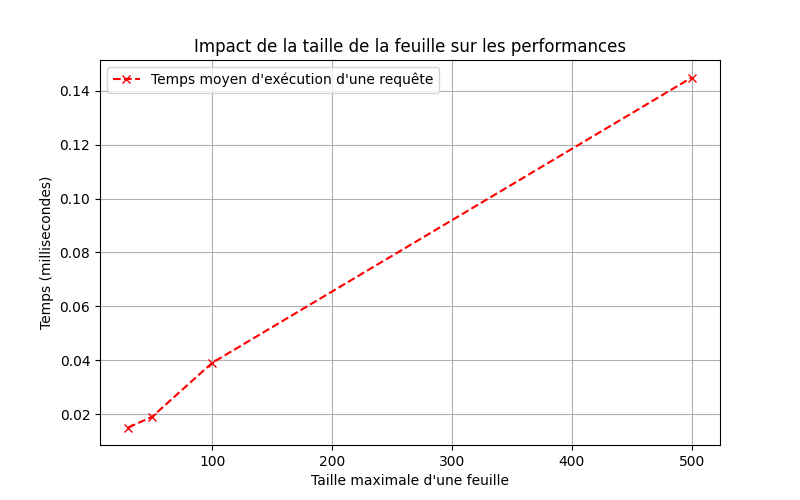
\includegraphics[width=0.8\textwidth]{images/average-query-time.png}
    \caption{Temps de requête moyen en fonction de la taille des feuilles}
    % \label{fig:leafsize}
\end{figure}


\newpage
\section{Le Connexion Scan Algorithm}
\subsection{Choix de l'algorithme}
Comme expliqué plus haut, pour résoudre le problème de recherche du plus court chemin, nous avons choisi d'implémenter le \emph{Connection Scan Algorithm} (\textbf{CSA}).
Cet algorithme est particulièrement adapté pour les réseaux de transport en commun, car il permet de trouver rapidement le meilleur chemin
entre deux arrêts en tenant compte des horaires de départ et d'arrivée. Le CSA a été conçu spécifiquement pour traiter les problèmes de planification d'itinéraires 
dans les systèmes de transport en commun. Cependant, au travers de nos recherches, nous avons découvert des alternatives algorithmiques comme \emph{Dijkstra} ou \emph{A*}.
Nous jugeons donc important de justifier notre choix.

\subsubsection{Fonctionnement}
\textbf{CSA}: Basé sur une approche de recherche de chemin utilisant une liste triée de connexions entre arrêts, et parcourant ces connexions linéairement.
Plus précisément, l'algorithme parcourt les connexions dans un ordre croissant suivant les temps de départ, en mettant à jour les meilleurs temps d'arrivée à 
chaque arrêt  \cite{dibbelt2017connection}.


\textbf{Dijkstra}: Cherche le plus court chemin en partant du noeud de départ et en explorant tous les voisins, en choisissant toujours le chemin avec 
le coût total le plus faible. Il utilise une file de priorité pour gérer les noeuds à explorer \cite{dijkstra1959note}.

\textbf{A*}: Une amélioration de Dijkstra ayant la particularité d'utiliser une heuristique afin de guider la recherche vers la destination. Nécessitant une
heuristique optimale pour garantir la complétude et l'optimalité de l'algorithme. Celui-ci est donc plus rapide que Dijkstra à condition d'avoir une heuristique
correcte \cite{astart2021literature}.

\subsubsection{Facilité d'implémentation avec GTFS}
\textbf{CSA}: Essentiellement une simple itération sur les connexions.

\textbf{Dijkstra}: Nécessite de transformer les données de GTFS en graphe temporel (chaque arrêt devient un noeud).
Cette implémentation est moins naturelle que celle du CSA mais marche tout aussi bien \cite{dijkstra1959note}.

\textbf{A*}: En plus de la construction du graphe temporel, il est primordial de définir une heuristique efficace.

\subsubsection{Complexité}
\textbf{CSA}: $O(n)$, où $n$ est le nombre de connexions (de manière naïve). Très rapide en pratique pour les requêtes \emph{earliest arrival} grâce au tri temporel. 
Cependant, il demande un tri réalisé au préalable, durant l'initialisation des données, déjà expliqué en détail à la section \hyperref[sec:complexitetempinit]{2.3.1.}
Pour le cas du CSA, nous verrons après qu'il y a encore des optimisations possibles pour diminuer la complexité temporelle.

\textbf{Dijkstra}: $O((V + E) \log V)$, où $V$ est le nombre de noeuds et $E$ le nombre d'arêtes du graphe temporel.

\textbf{A*}: $O((V + E) \log V)$, mais dépend de la qualité de l'heuristique.

\subsubsection{Choix final}
Les algorithmes Dijkstra et A* utilisent donc des structures de données plus complexes comme des graphes temporels et des files de priorité. Ceci implique donc
un certain niveau de complexité supplémentaire dans l'implémentation.

Nous avons donc décider de miser sur la simplicité d'implémentation et la rapidité de l'algorithme CSA, celui-ci
se basant essentiellement sur une liste de connexions triées. De plus, celui-ci est par défaut adapté aux fichiers GTFS et les horaires de transports publics.
nous avons choisi d'implémenter le \emph{Connection Scan Algorithm} (\textbf{CSA}) pour notre projet \cite{linkGTFSCSA}.

\subsection{Explication et description de l'algorithme}
Le \emph{Connection Scan Algorithm} est une méthode efficace pour résoudre les problèmes de planification d'itinéraires dans 
les réseaux de transports en commun basés sur des horaires, comme les trains et les bus. Contrairement aux algorithmes classiques 
qui utilisent une file de priorité (comme Dijkstra), le CSA se base sur une liste triée de tous les transports en commun, classés par 
leur heure de départ.

Il parcourt cette liste de manière séquentielle pour déterminer rapidement les meilleures connections possibles pour atteindre une 
destination dans un délai optimal ou avec le moins de changements de véhicule.

\subsection{Structures de l'algorithme et implémentation}
L'algorithme est stocké dans une classe \texttt{PathFinder} contenant la méthode findPath, qui implémente l'algorithme CSA.
\begin{table}[h]
  \centering
  \begin{tabular}{|l|l|p{8cm}|}
  \hline
  \textbf{Attribut/Méthode} & \textbf{Type/Retour} & \textbf{Description} \\
  \hline
  stopMap & Map$<$String, Stop$>$ & Map contenant les arrêts, indexés par leur identifiant. \\
  tripMap & Map$<$String, Trip$>$ & Map contenant les trajets, indexés par leur identifiant. \\
  routeMap & Map$<$String, Route$>$ & Map contenant les routes, indexées par leur identifiant. \\
  connexions & List$<$Connexion$>$ & Liste des connexions disponibles. \\
  \hline
  findPath & void & Implémente l'algorithme pour trouver le meilleur chemin dans le graphe. \\
  \hline
  \end{tabular}
  \caption{Classe PathFinder sans les méthodes annexes}
\end{table}

\subsection{Pseudo-code sans la marche à pied et autres optimisations}
\begin{algorithm}[H]
  \footnotesize
  \SetAlgoNlRelativeSize{-1}
  \DontPrintSemicolon
  \KwIn{start, destination, time}
  \KwOut{Affiche le chemin optimal ou un message d'erreur}
  \tcp{La liste de connexions est triée par heure de départ préalablement durant le parsing}
  
  \ForEach{stopId dans tous les arrêts}{
    shortestPath[stopId] $\gets \infty$ \;
  }
  \ForEach{startingStop dans startingStops}{
    shortestPath[startingStop] $\gets$ userStartTime \;
  }
    
  \ForEach{connexion \texttt{c} dans \texttt{connexions}}{
      \If{\texttt{shortestPath[dep]} $\leq$ \texttt{depTime} \textbf{et} \texttt{shortestPath[arrive]} $>$ \texttt{arrTime}}{
          Mettre à jour \texttt{shortestPath[arrive]} et \texttt{previousConnection[arrive]} \;
      }
      \ForEach{walk depuis \texttt{depart}}{
          \If{\texttt{shortestPath[walkArr]} $>$ \texttt{walkTime}}{
              Mettre à jour \texttt{shortestPath[walkArr]} et \texttt{previousConnection[walkArr]} \;
          }
      }
  }

  \texttt{currentStop} $\gets$ \texttt{end\_stop} \;
  \While{\texttt{currentStop} dans \texttt{previousConnection}}{
      Ajouter la connexion à \texttt{path} au début \;
      \texttt{currentStop} $\gets$ origine de la connexion \;
  }
  
  \text{Afficher le chemin trouvé} \;
  
  \caption{CSA --- Recherche de chemin entre deux arrêts sans marche à pied}
  \end{algorithm}
    
\subsection{Complexité sans la marche à pied et autres optimisations}
Une fois l'initialisation des données terminée (cf. section \hyperref[sec:init]{2}), l'algorithme CSA est donc relativement direct à implémenter.
Il débute par le parcours de toutes les connexions une par une. Cette opération est naturellement linéaire, $O(n)$, où $n$ est le nombre de connexions.
Cette complexité est particulièrement avantageuse pour les grands ensembles de données, car elle permet un traitement efficace 
des requêtes après le prétraitement initial.

Tout ceci nous amène donc à une complexité totale de $O(n)$ pour la recherche de chemin, où $n$ est le nombre de connexions.

Notons tout de même le fait que cette compléxité est valable uniquement dans le cas où nous ne considérons pas les transferts à pied, chose que nous
explicitons dans la section suivante.

\subsection{Pseudo-code avec la marche à pied et algorithme optimal}
\begin{algorithm}[H]
  \footnotesize
  \SetAlgoNlRelativeSize{-1}
  \DontPrintSemicolon
  \KwIn{startName, destinationName, userTime}
  \KwOut{Affiche le chemin optimal ou un message d'erreur}

  \ForEach{stopId dans tous les arrêts}{
    shortestPath[stopId] $\gets \infty$ \;
  }
  \ForEach{startingStop dans startingStops}{
    shortestPath[startingStop] $\gets$ userStartTime \;
  }

  bestArrivalTime $\gets \infty$   \tcp{Initialisation du meilleur temps d'arrivée}\;

  \tcp{Starting criterion}
  startIndex $\gets$ index de la première connexion avec depTime >= userStartTime (recherche dichotomique) \;

  \For{i $\gets$ startIndex \KwTo connexions.size()}{
    c $\gets$ connexions[i] \;
    \If{c.depTime > bestArrivalTime}{
      \textbf{break} \tcp*{Stopping criterion --- plus de chemin possible}
    }

    \If{shortestPath[c.dep] $\leq$ c.depTime \textbf{et} shortestPath[c.arr] $>$ c.arrTime}{
      shortestPath[c.arr] $\gets$ c.arrTime \;
      previousConnection[c.arr] $\gets$ c \;

      \If{c.arr $\in$ endStops \textbf{et} c.arrTime < bestArrivalTime}{
        bestArrivalTime $\gets$ c.arrTime \;
      }

      \ForEach{walk $\in$ walks depuis c.arr}{
        walkArr $\gets$ walk.destination \;
        walkTime $\gets$ c.arrTime + walk.duration \;
        \If{shortestPath[walkArr] $>$ walkTime}{
          shortestPath[walkArr] $\gets$ walkTime \;
          previousConnection[walkArr] $\gets$ \texttt{Connexion de type marche} \;
        }
      }
    }
  }

  \While{\texttt{currentStop} dans \texttt{previousConnection}}{
      Ajouter la connexion à \texttt{path} au début \;
      \texttt{currentStop} $\gets$ origine de la connexion \;
  }
  \text{Afficher le chemin trouvé} \;
  
  \caption{CSA --- Recherche de chemin avec critères d'arrêt et marches à pied}
\end{algorithm}


\subsection{Complexité avec la marche à pied et algorithme optimal}
Comme expliqué dans la sous-section précédente, l'algorithme de base est en $O(n)$, avec $n$ est le nombre de connexions. Mais, il n'est clairement pas logique
de considérer un voyage où nous ne marchons pas du tout. C'est pourquoi nous devons aussi prendre en compte les transferts à pied. Lors de l'exécution de
l'algorithme, à chaque itération, autrement dit à chaque connexion, nous devons vérifier si l'arrêt de départ concerné possède des arrêts voisins à une distance
donnée (500m dans notre cas, cf. \hyperref[sec:complexitetempinit]{2.3.1.}). Un transfert entre deux arrêts voisins est représenté comme un \emph{Walk}, une
classe décrite dans la section \hyperref[sec:walk]{2.2.3.}. Donc, pour chaque arrêt nous allons parcourons l'ensemble des transferts à pied disponibles.
En prenant $\bar{m}$ comme nombre moyen de transferts à pied moyen, nous avons une complexité totale de $O(n * \bar{m})$, avec $n$ étant toujours le nombre de connexions.

Nous pourrions croire que la complexité de l'algorithme avec les transferts à pied se rapproche de $O(n^2)$, mais ce n'est pas le cas. Pour répondre à cette incertitude,
nous avons tout simplement calculé la moyenne du nombre de transferts à pied par arrêt à l'aide d'un script Python. Ceci nous a mené à une valeur de 7 voisins dans un
rayon de 500 mètres par arrêt. Nous concluons donc que, avec un nombre de connexions étant de l'ordre de dizaines de millions, $\bar{m}$ est négligeable par rapport à $n$ et
nous arrivons à une complexité totale de $O(n)$.

\subsubsection{Optimisations}
Comme montré ci-dessus, l'algorithme n'est pas exactement linéaire. Nous avons donc décidé d'implémenter deux optimisations afin d'améliorer la vitesse de l'algorithme.
\begin{itemize}
    \item \textbf{Starting criterion:} Nous utilisons l'algorithme élémentaire qu'est la recherche dichotomique (en $O(\log n)$), pour trouver le premier arrêt 
    qui est supérieur ou égal à l'heure de départ. Ceci nous évite le parcours toutes les connexions en nous permettant de commencer à partir de l'indice trouvé.
    À travers ce procédé, nous de réduisons le nombre d'itérations nécessaire pour trouver le chemin optimal. En effet, pour une requête de trajet débutant en fin
    de journée, pourquoi itérer dans les premières connexions ? Ceci est tout naturellement inutile. Grâce à cela, l'algorithme passe de $O(n)$ à $O(n - k)$ 
    avec $k$ le nombre de connexions avant l'heure de départ. La variable $k$ pouvant prendre des valeurs de $0$ à $n$, elle n'est pas négligeable dans le calcul
    de complexité totale. En conclusion, cela nous permet de grandement réduire le temps d'exécution de l'algorithme, et encore plus si l'heure de départ est
    est élevée. Toutefois, si l'heure entrée par l'utilisateur est la première dans la liste de connexion, la complexité ne change pas et reste $O(n)$ car nous
    devons parcourir toutes les connexions.
    \item \textbf{Stopping criterion:} Cette seconde optimisation nous permet d'arrêter l'algorithme soit lorsque la destination atteinte, soit lorque toutes 
    les connexions possibles ont été explorées. Cela nous éviter le parcours inutile des connexions qui ne contribuent pas à améliorer le chemin trouvé. 
    En pratique, dans le cas où l'heure d'arrivée à un arrêt est déjà optimale (c'est-à-dire qu'aucune connexion ultérieure ne peut améliorer cette heure), cela signifie
    que nous pouvons ignorer les connexions restantes. Cette optimisation réduit potentiellement une fois de plus le nombre d'itérations nécessaires afin de trouver le
    chemin optimal. En ce qui concerne la complexité, en prenant la complexité de base de l'algorithme, nous passons de $O(n)$ à $O(n - j)$ où $j$ est le nombre de 
    connexions que nous avons pu soustraire. Ceci nous permet une fois de plus d'avoir de meilleures performances globale.
\end{itemize}

En somme, en assemblant nos deux optimisations, nous obtenons une complexité totale de $O(n - k - j)$ pour le coeur de l'algorithme.

Il reste finalement l'étape de la reconstruction du chemin. Celle-ci se fait en parcourant les connexions de path et donc nous sommes en $\Theta(p)$ ou p est le nombre de connexions dans path.
TODO TODO TODO @ROMAIN

Il existe une troisième optimisation du CSA s'appellant `Limited Walking'. Malheureusement, celle-ci s'est révélée plus compliquée à mettre en place et, par manque de temps, 
nous n'avons pas eu l'occasion de l'implémenter. % TODO: détailler tout de même en qlq mots ?? 

\subsection{Chiffres concrets}
\begin{figure}[H]
  \centering
  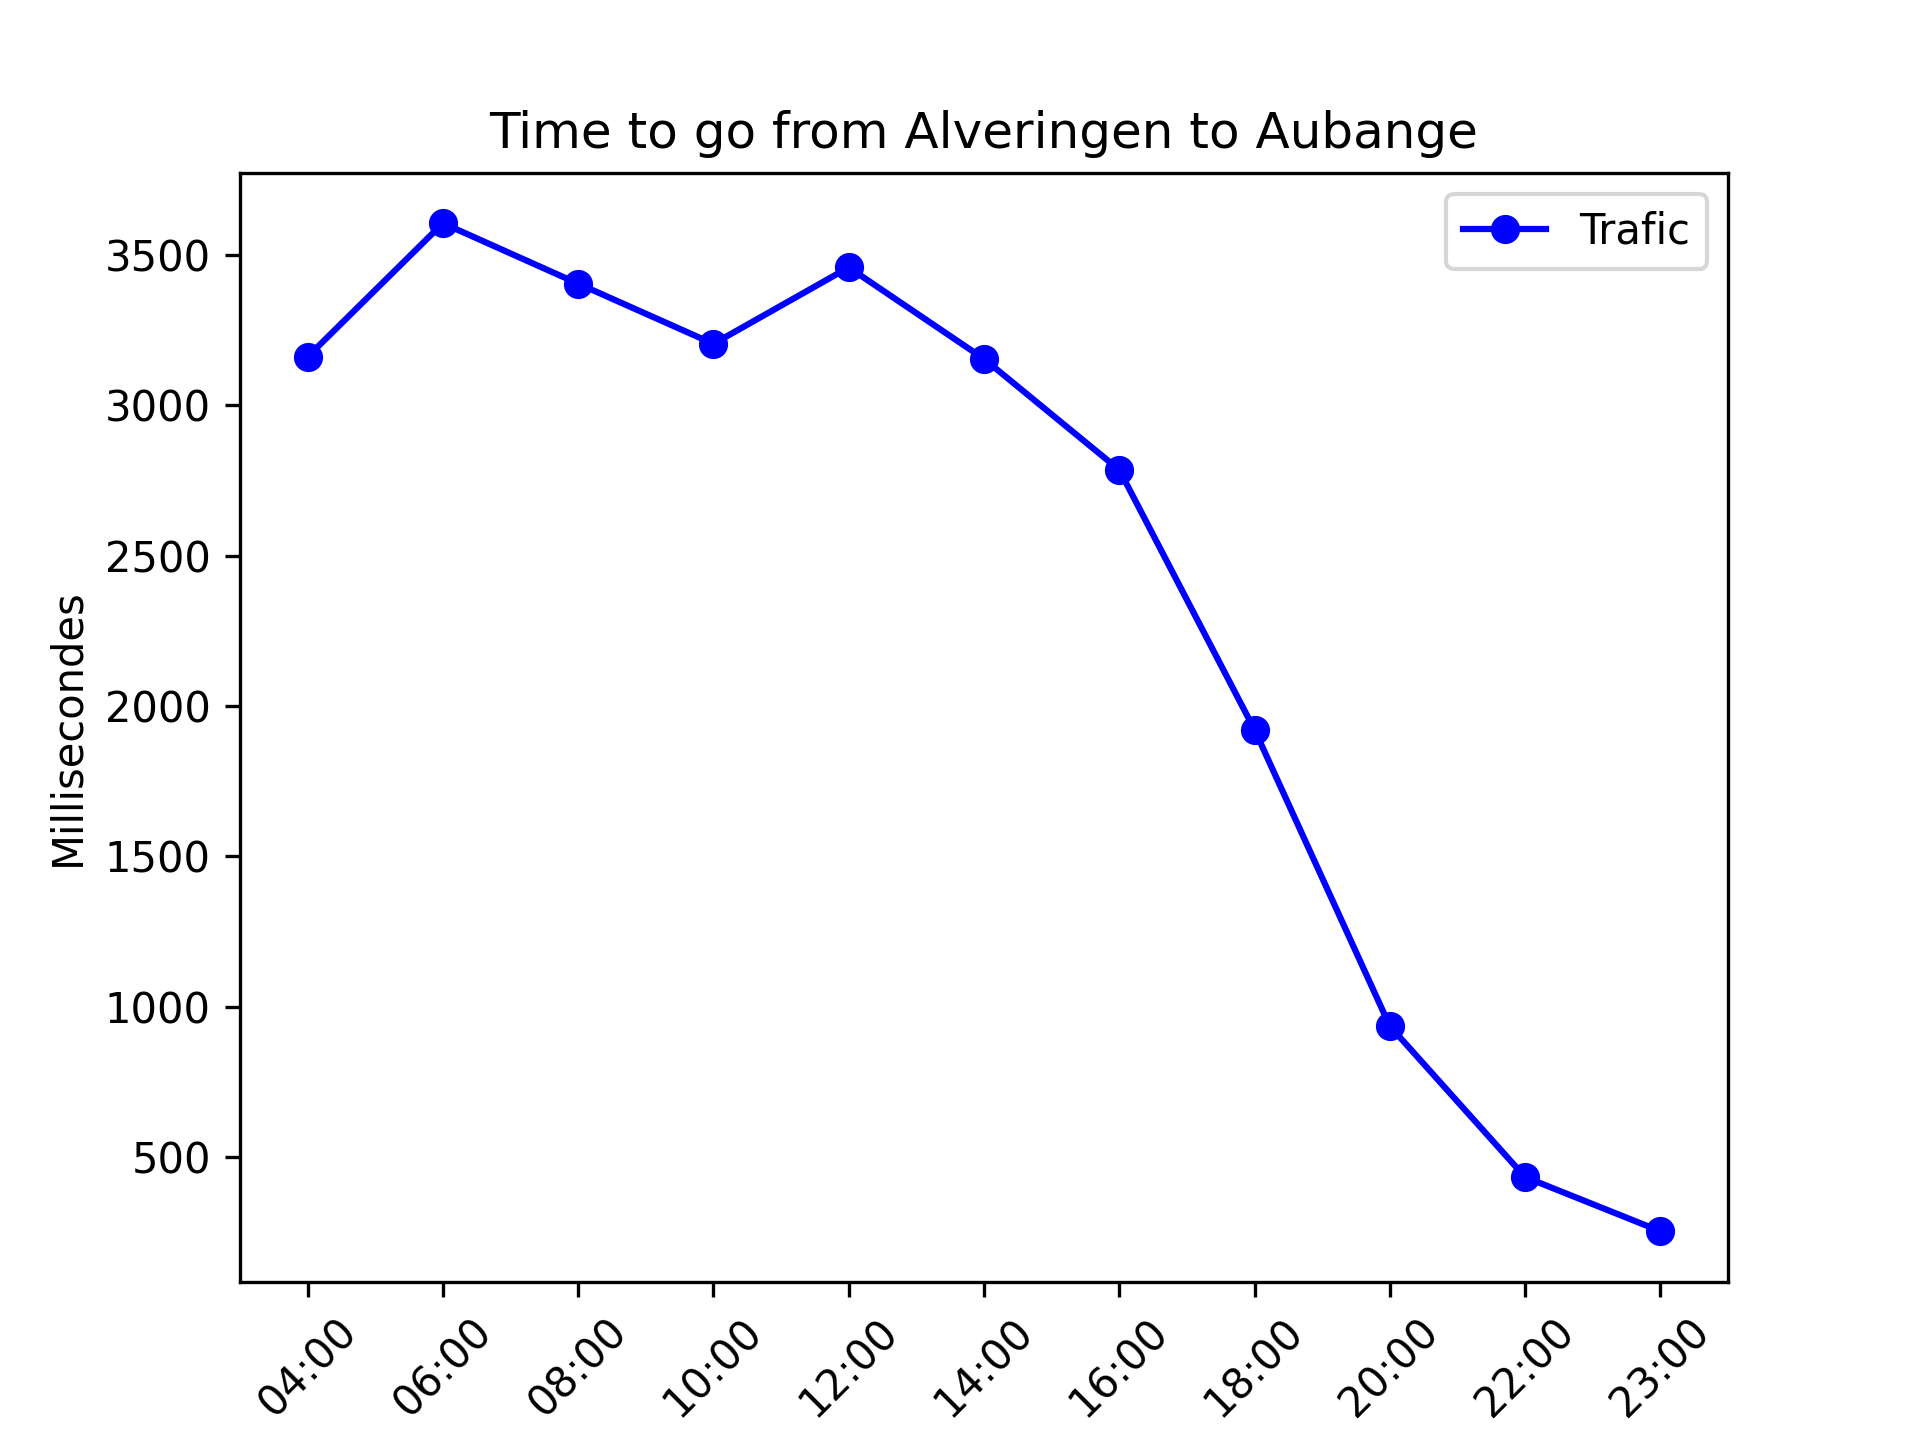
\includegraphics[width=0.8\textwidth]{graphique_traffique}
  \caption{Graphique du temps d'exécution en fonction de l'heure de départ.}
  \label{fig:graphique_traffique}
\end{figure}
De part ce graphe, nous pouvons voir que le temps d'exécution de l'algorithme est relativement constant jusqu'à 16h, puis grâce au Starting criterion,
l'algorithme devient de plus en plus rapide. En effet, à partir de 16h, il y a moins de connexions et il arrive a chaque fois à trouver le chemin optimal en mois d'une seconde.
Nous pouvons aussi parler du Stopping criterion, qui lui permet de ne pas parcourir toutes les connexions et donc de ne pas perdre de temps à chercher des connexions inutiles.
Bien que nous ne puissions pas le voir sur le graphe, il est tout de même présent et permet de réduire le temps d'exécution de l'algorithme.

\section{Classes utilisées}

\section{Conclusiion}


\section{Sources-bibliographie}
\cite{dibbelt2017connection} 
\cite{butts2020raptor}
\cite{epfl2024cs108}
\cite{transnetlabCSA}
\cite{gtfsReference}
\cite{futura2009distance}
\cite{geeko2018distance}
\cite{geeksforgeeks_haversine}
\cite{wikipedia_geohash}
\cite{mattaparthi2024ballkd}
\cite{fieldsend_onlineballtree}
\cite{woltmann2025astar}
\cite{wikipedia_astar}
\cite{geeksforgeeks_astar}
\cite{wikipedia_dijkstra}
\cite{baeldung_collections_sort}
\cite{wikipedia_timsort}

\printbibliography


\end{document}